\section[Installation de Docker]{Installation de Docker 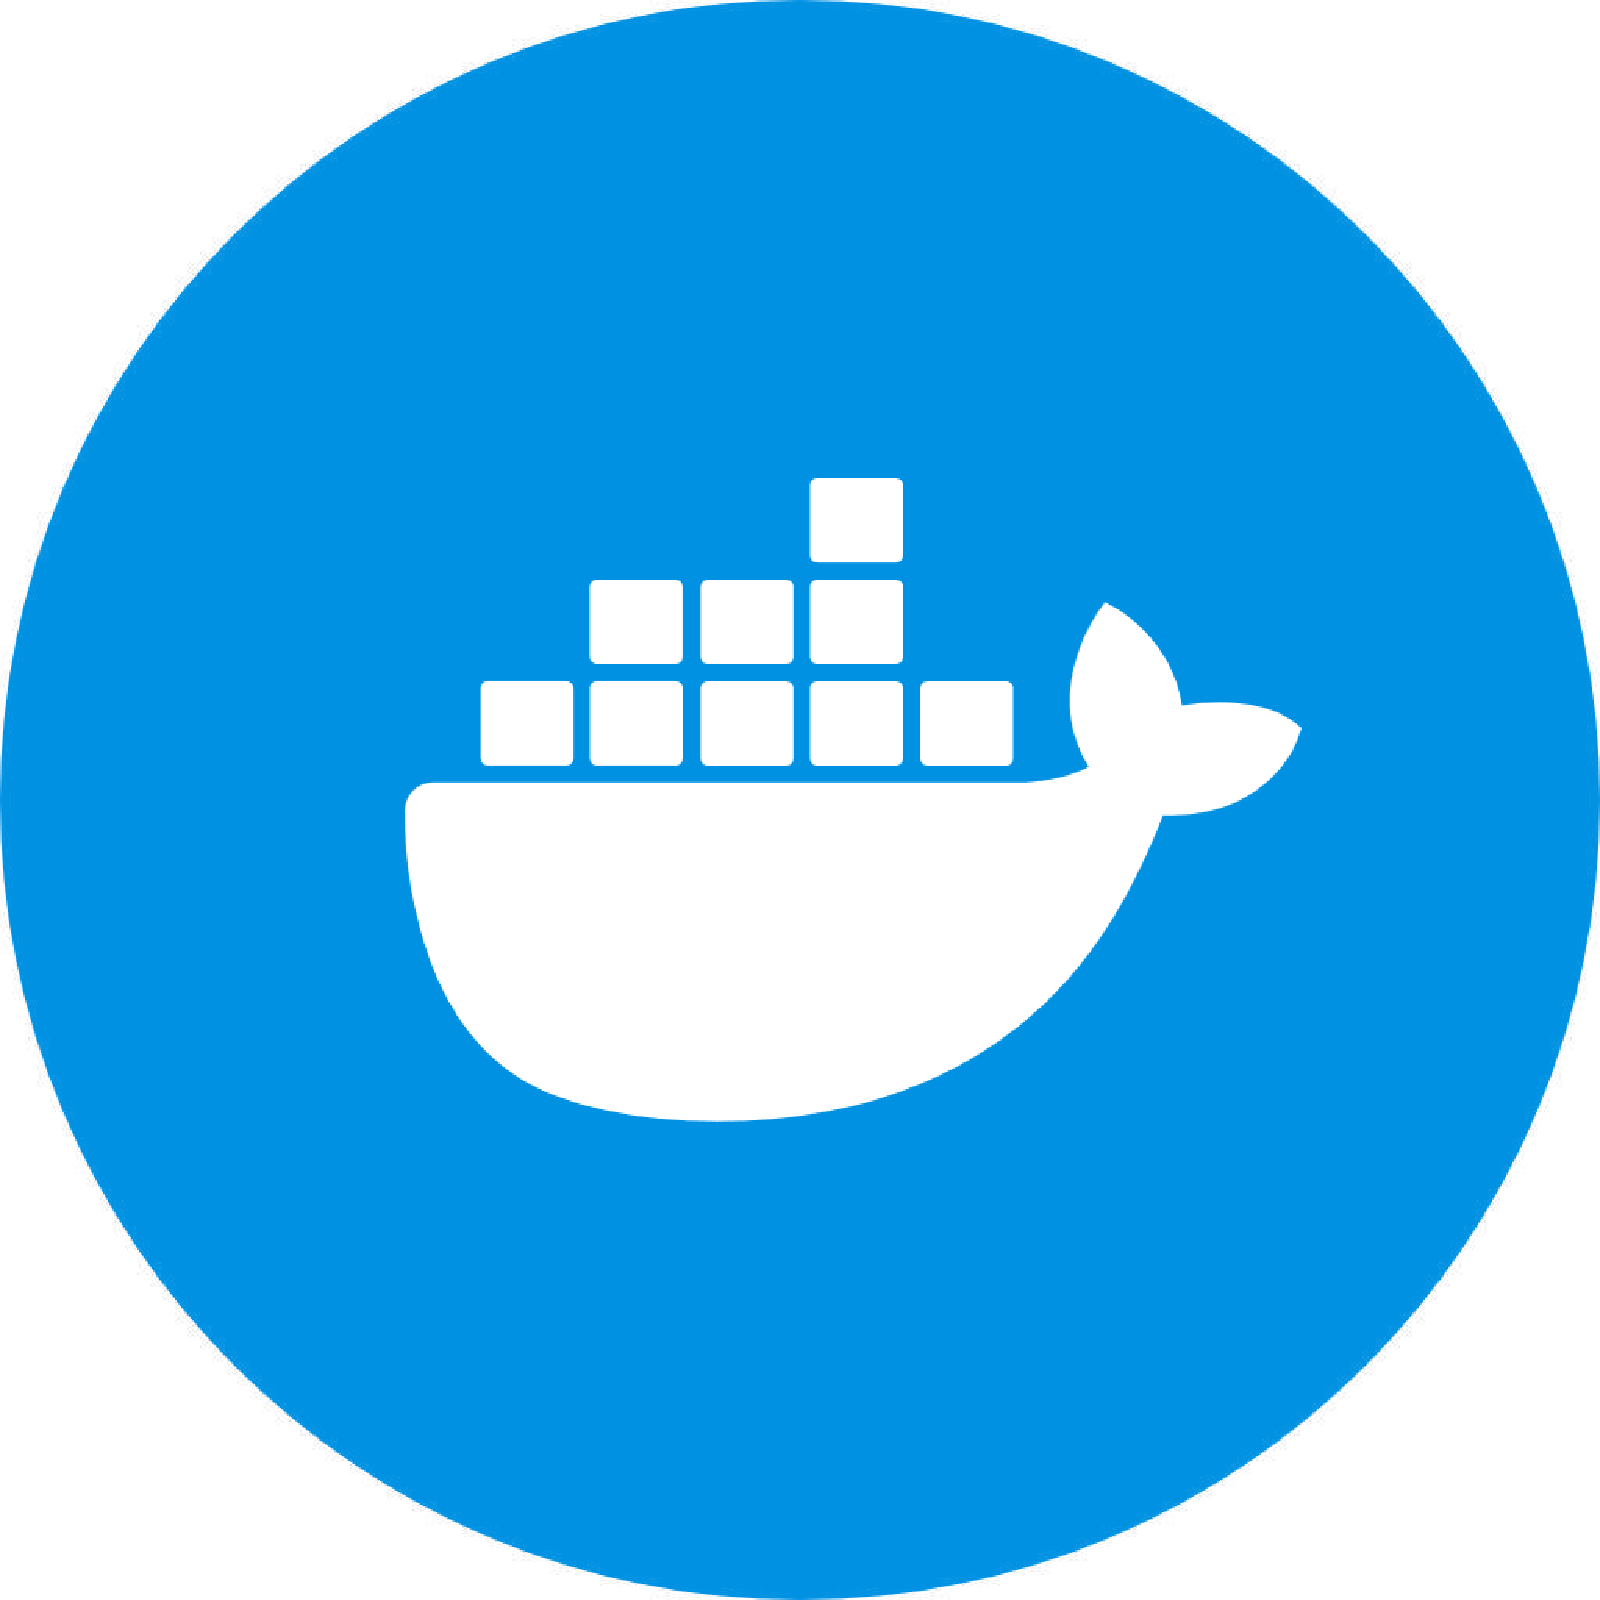
\includegraphics[height=15pt]{figures-logos/docker.pdf}}

Choisissez la section correspondant à votre système d'exploitation:

\begin{figure}[!h]
    \centering
    \begin{minipage}{0.32\textwidth}
        \centering
        \hyperref[sec:installation_linux]{
\includegraphics[scale=0.05]{Images_formation/LinuxLogo.pdf}}
        \caption*{\underline{Linux}: \textsc{section~\ref{sec:installation_linux}}}
    \end{minipage} 
    \begin{minipage}{0.32\textwidth}
        \centering
        \hyperref[sec:installation_windows]{
\includegraphics[scale=0.020]{Images_formation/WindowsLogo.pdf}}
        \caption*{\underline{Windows}: \textsc{section~\ref{sec:installation_windows}}}
    \end{minipage}
    \begin{minipage}{0.32\textwidth}
        \centering
        \hyperref[sec:installation_macos]{
\includegraphics[scale=0.025]{Images_formation/MacosLogo.pdf}}
        \caption*{\underline{MacOS}: \textsc{section~\ref{sec:installation_macos}}}
    \end{minipage}
\end{figure}
\subsection[Installation Linux]{Installation \linux{}\label{sec:installation_linux}}

    L'Installation \linux{} nécessite de suivre quelques étapes de plus que pour l'Installation \macos{} ou \windows{}.\\
    \begin{itemize}
    
        \item[1.] Mettez à jour l'index des paquets apt et des paquets d'installation pour permettre à apt d'utiliser un dépôt sur HTTPS:
        
            \begin{lstlisting}
                sudo apt-get update
            \end{lstlisting}

        \item[2.] Installez les dépendances de \docker{}:

            \begin{lstlisting}
                sudo apt-get install \
                    ca-certificates \
                    curl \
                    gnupg \
                    lsb-release
            \end{lstlisting}

        \item[3.] Ajoutez la clé GPG officielle de \docker{}:

            \begin{lstlisting}
                sudo mkdir -m 0755 -p /etc/apt/keyrings

                curl -fsSL https://download.docker.com/linux/ubuntu/gpg | 
                sudo gpg --dearmor -o /etc/apt/keyrings/docker.gpg
            \end{lstlisting}

        \item[4.] Configurez le répertoire:\\

            \begin{footnotesize}
                \textit{\textdollar(lsb\_release -cs)} doit dans quelques cas être remplacé par votre version de distribution \linux{}.\\
                Dans l'installation de référence on a remplacé par \textit{jammy}.
            \end{footnotesize}
            \begin{lstlisting}
                echo \
                "deb [arch=\$(dpkg --print-architecture) 
                signed-by=/etc/apt/keyrings/docker.gpg] https://download.docker.com/linux/ubuntu \
                \$(lsb_release -cs) stable" 
                | sudo tee /etc/apt/sources.list.d/docker.list > /dev/null
            \end{lstlisting}

        \item[5.] Verifiez que le répertoire est bien configuré:

            \begin{lstlisting}
                sudo apt-get update
            \end{lstlisting}    

        \item[6.] Installez Docker Engine, conteneurd, et Docker Compose:

            \begin{lstlisting}
                sudo apt-get install docker-ce docker-ce-cli 
                conteneurd.io docker-buildx-plugin docker-compose-plugin
            \end{lstlisting}
            \begin{footnotesize}
                Vous pouvez tester votre installation avec la commande: \textit{sudo docker run hello-world}
            \end{footnotesize}

            \bigskip
        \item[7.] Installez \dockerdesktop{}:

        
            \begin{footnotesize}
                Téléchargez \href{https://desktop.docker.com/linux/main/amd64/docker-desktop-4.17.0-amd64.deb?utm_source=docker&utm_medium=webreferral&utm_campaign=docs-driven-download-linux-amd64}{Docker Destop} et installez le avec la commande:
            \end{footnotesize}

            \begin{lstlisting}
                sudo apt-get install ./docker-desktop-<version>-<arch>.deb
            \end{lstlisting}

    \end{itemize}

    \bigskip

    \begin{footnotesize}
        L'Installation de référence pour ce guide a été faite sur une distribution \linux{} Mint (distibution basé sur \ubuntu{})\\
    \end{footnotesize}

    \hyperref[sec:suite_installation]{Pour passer à la suite}

\newpage

\subsection[Installation Windows]{Installation \windows{}\label{sec:installation_windows}}

    \subsubsection[Prérequis][fr.wikipedia.org/wiki/Windows_Subsystem_for_Linux]{Prérequis: WSL2}

    Pour utiliser \dockerdesktop, il est fortement conseillé d'utiliser \href{https://learn.microsoft.com/fr-fr/windows/wsl/install}{WSL2}. C'est une application \windows{} permettant d'installer un environnement \linux{} avec la distribution de votre choix nativement sous \windows{}. 

    Pour l'installer, il suffit de lancer \verb|wsl --install| dans le terminal de \windows{} de base ou \texttt{Powershell}\footnote{Attention, le terminal choisi doit être exécuté en tant qu'administrateur !}. Par défaut, cette commande installera \ubuntu{} comme système \linux. Pour d'avantage d'informations conçernant l'installation de WSL2, consultez le lien vers la page officielle de Microsoft. Si tout se passe bien vous devriez recevoir le message suivant:

    \begin{figure}[!th]
        \centering
        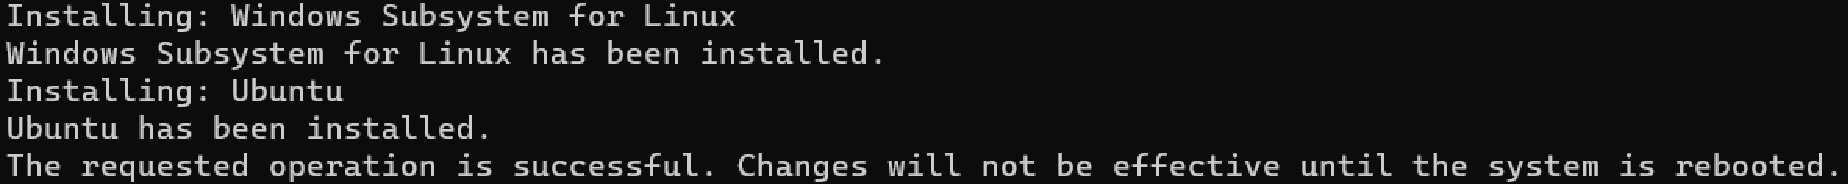
\includegraphics[width=0.75\textwidth]{Images_formation/ubuntu_installation.pdf}
    \end{figure}

    Après avoir redémaré votre PC, la fenêtre suivante devrait apparaitre. Si ce n'est pas le cas, cherchez \texttt{wsl.exe} dans la barre de recherche windows et lancez le terminal.

    \begin{figure}[!th]
        \centering
        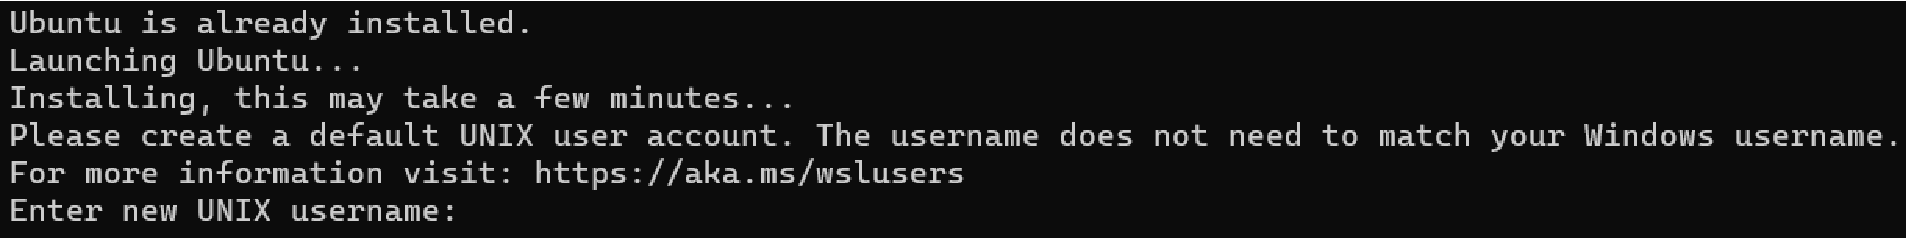
\includegraphics[width=0.75\textwidth]{Images_formation/user_creation.pdf}
    \end{figure}

    Ici, vous devez créer un utilisateur ainsi qu'ajouter un mot de passe\footnote{Lorsque vous tapez votre mot de passe, il est normal que les charactères ne s'affichent pas.}. Attention, vous devrez utiliser votre mot de passe de temps en temps, donc ne l'oubliez pas!

    Enfin, exécutez \verb|sudo apt update| et puis \verb|sudo apt upgrade| afin d'être sur que votre environnement est à jour.

    Une fois ces étapes effectuées sans accroc, vous pouvez passer à l'installation de \dockerdesktop{} à proprement parler.

    \subsubsection[Installation de Docker Desktop]{Installation de \dockerdesktop}
    
    \begin{itemize}
        \item[1.] Téléchargez \href{https://desktop.docker.com/win/main/amd64/Docker%20Desktop%20Installer.exe}{\dockerdesktop{}}
        
        \item[2.] Exécutez le fichier d'installation \verb|.exe|
        
        \item[3.] Vérifiez l'installation en lançant votre environnement \verb|wsl| et en tapant la commande suivante:
        \begin{lstlisting}
            docker
        \end{lstlisting}
    \end{itemize}

    \docker{} et wsl2 sont totalement compatibles. C'est pourquoi vous devez cocher l'option ``use WSL2'' pendant l'installation. 

    \hyperref[sec:suite_installation]{Pour passer à la suite}

\newpage
\subsection[Installation MacOS]{Installation \macos{}\label{sec:installation_macos}}

    \begin{itemize}
        \item[1.] Téléchargez \dockerdesktop{} \href{https://desktop.docker.com/mac/main/arm64/Docker.dmg?utm_source=docker&utm_medium=webreferral&utm_campaign=dd-smartbutton&utm_location=module}{Apple Chip} ou \href{https://desktop.docker.com/mac/main/amd64/Docker.dmg?utm_source=docker&utm_medium=webreferral&utm_campaign=dd-smartbutton&utm_location=module}{Intel Chip}.
        \item[2.] Installez \dockerdesktop{} dans le dossier \verb|application|.
    \end{itemize}

    \hyperref[sec:suite_installation]{Pour passer à la suite}

\newpage

\subsection[Aperçu]{Aperçu\label{sec:suite_installation}}
    Si tout s'est bien passé, vous êtes en mesure de lancer \dockerdesktop{}. Vous avez donc le panneau de contrôle de \dockerdesktop{} qui devrait ressembler à ça:\\
    \begin{figure}[h]
        \centering
        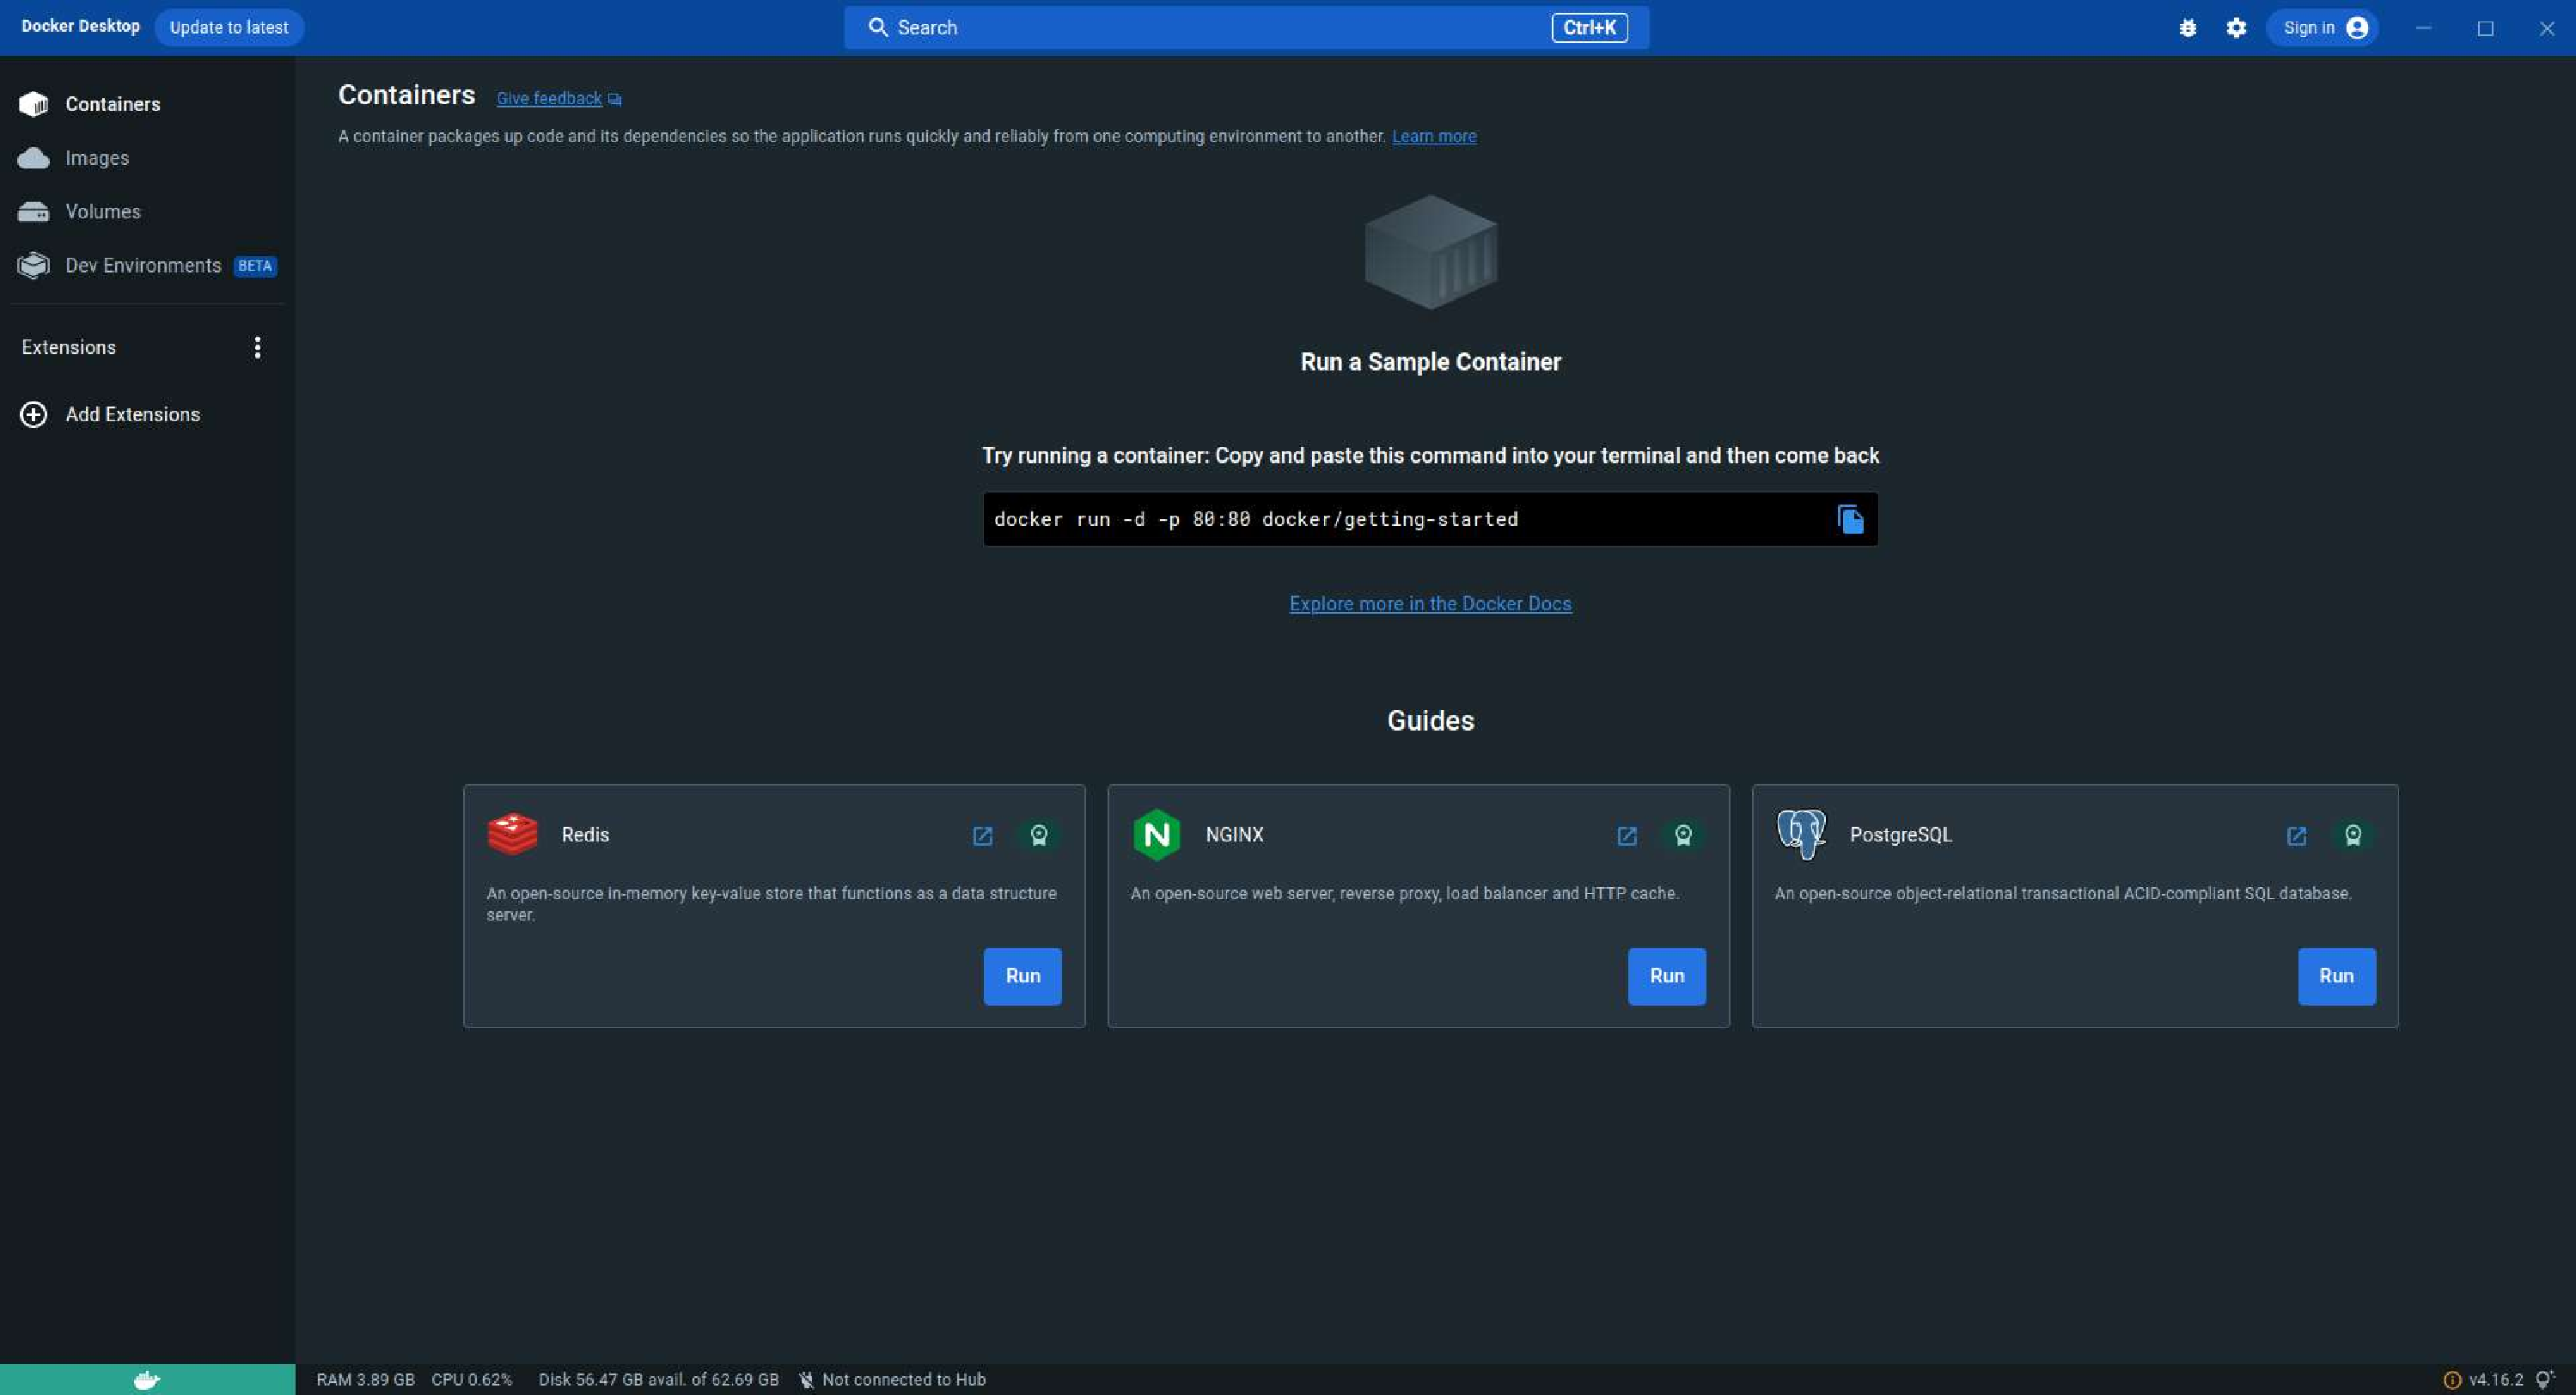
\includegraphics[width=0.7\textwidth]{Images_formation/PanelDocker.pdf}
    \end{figure}

    Vous pouvez voir différents onglets sur la gauche:

    \begin{itemize}
        \item Conteneurs: Cet onglet va contenir tous les conteneurs que vous avez créés. Les conteneurs sont en quelque sorte des images déployées et exécutées lorsque \docker{} tourne.
        \item Images: Cet onglet va contenir toutes les images d'installation des services installés dans nos conteneurs. Les images décrivent l'environnement du serveur, les packages installés et toutes les configurations de celui-ci.
        \item Volumes: Cet onglet contient les volumes liés aux services qui contiennent les données de nos applications. Les volumes servent à conserver les données des bases de données lorsque nous éteignons un container et qu'on le relance.
        \item Dev Environnements: une \texttt{feature} très intéressante permettant de créer des environnements de développement \footnotesize{\href{https://docs.docker.com/desktop/dev-environments/}{(plus d'informations)}}.
    \end{itemize}

\subsection[VS Code]{Utilisez \vscode!! (surtout \windows)}
    Enfin, pour utiliser tout ce que nous venons d'installer, il faut un éditeur de code efficace. \href{https://code.visualstudio.com/}{\vscode{}} permet, via ses extensions d'interagir avec \docker{} et WSL2 en parfaite harmonie, c'est pourquoi nous le recommandons CHAUDEMENT. 

    \begin{wrapfigure}{r}{0.2\textwidth}
        \centering
        \vspace*{-0.5cm}
        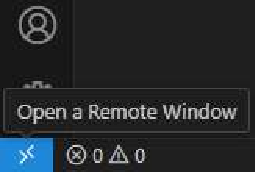
\includegraphics[width=0.2\textwidth]{Images_formation/connect_to_wsl.pdf}
    \end{wrapfigure}
    Une fois \vscode{} installé, ajoutez les extensions WSL (de Microsoft) et Docker (de Microsoft également). Une fois cela fait, cliquez sur le petit carré montré ci-joint.

    Ensuite, sélectionnez \verb|Connect to WSL|. Enfin, \texttt{File} $\rightarrow$ \texttt{Open Folder\ldots} et appuyez sur ok. Normalement, vous devriez vous trouver dans le dossier source.
